%\documentclass[smaller,handout]{beamer}
\documentclass[smaller]{beamer}

\usepackage{amsfonts}
\usepackage{amssymb}
\usepackage{amsmath}
\usepackage{epsfig}
\usepackage{graphicx}

\def\F{{\cal F}}
\def\X{{\cal X}}
\def\Y{{\cal Y}}
\def\Z{{\cal Z}}
\def\P{{\mathbb P}}
\def\R{{\mathbb R}}
\def\E{{\mathbb E}}
\def\bZ{{\mathbb Z}}
\def\darkred{\color{red!70!black}}
\def\darkgreen{\color{green!60!black}}
\def\learn{{\mbox{LEARN}}}
\def\err{{\mbox{err}}}
\def\bI{{\tilde{I}}}
\def\dis{{\mbox{DIS}}}

\DeclareMathOperator*{\argmin}{arg\,min}
\DeclareMathOperator*{\argmax}{arg\,max}

%\usepackage{pgfpages}
%\pgfpagesuselayout{4 on 1}[letterpaper,border shrink=5mm,landscape]

%\usepackage{beamerarticle}

\mode<presentation>
{
  \usetheme{default}
%  \setbeamercovered{transparent}
  % or whatever (possibly just delete it)
}


\usepackage[english]{babel}
% or whatever

\useinnertheme{circles}
\usefonttheme{structurebold}

%\usepackage[latin1]{inputenc}
% or whatever

%\usepackage{times}
%\usepackage[T1]{fontenc}
% Or whatever. Note that the encoding and the font should match. If T1
% does not look nice, try deleting the line with the fontenc.

\title{Classification with generative models II}

\author{DSE 210}
% - Give the names in the same order as the appear in the paper.
% - Use the \inst{?} command only if the authors have different
%   affiliation.

%\institute{University of California, San Diego}

\date{}

% If you wish to uncover everything in a step-wise fashion, uncomment
% the following command: 

%\beamerdefaultoverlayspecification{<+->}
\setbeamertemplate{navigation symbols}{}

\def\vone{{\vskip.1in}}
\def\v2{{\vskip.2in}}
\def\bR{{\mathbb R}}
\def\R{{\mathbb R}}
\def\eps{{\epsilon}}
\def\E{{\mathbb E}}
\def\epso{{\epsilon_o}}
\def\nicered{{\color{red!70!black}}}
\def\pr{{\mbox{\rm Pr}}}

\setbeamercolor{title}{fg=red!80!black,bg=red!20!white}
\setbeamercolor{author}{fg=blue!80!black}

\begin{document}

% *** TITLE ***
\begin{frame}
  \titlepage
\end{frame}

% *** CLASSIFICATION WITH PARAMETRIZED MODELS ***
\begin{frame}
\frametitle{Classification with parametrized models}

{\darkred 
Classifiers with a fixed number of parameters can represent a limited set of functions. Learning a model is about picking a good approximation.}

\v2
{\darkgreen Typically the $x$'s are points in $p$-dimensional Euclidean space, $\R^p$.}

\begin{center}
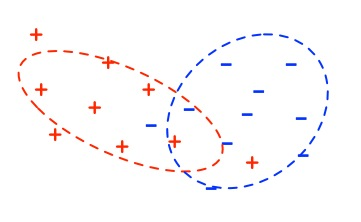
\includegraphics[width=1.75in]{generative.jpg}
\hskip.5in
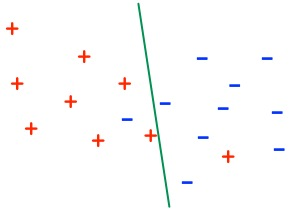
\includegraphics[width=1.75in]{discriminative.jpg}
\end{center}

Two ways to classify:
\begin{itemize}
\item \alert{\bf Generative}: model the individual classes.
\item \alert{\bf Discriminative}: model the decision boundary between the classes.
\end{itemize}

\end{frame}

% *** THE BAYES-OPTIMAL PREDICTION ***
\begin{frame}
\frametitle{The Bayes-optimal prediction}

\begin{center}
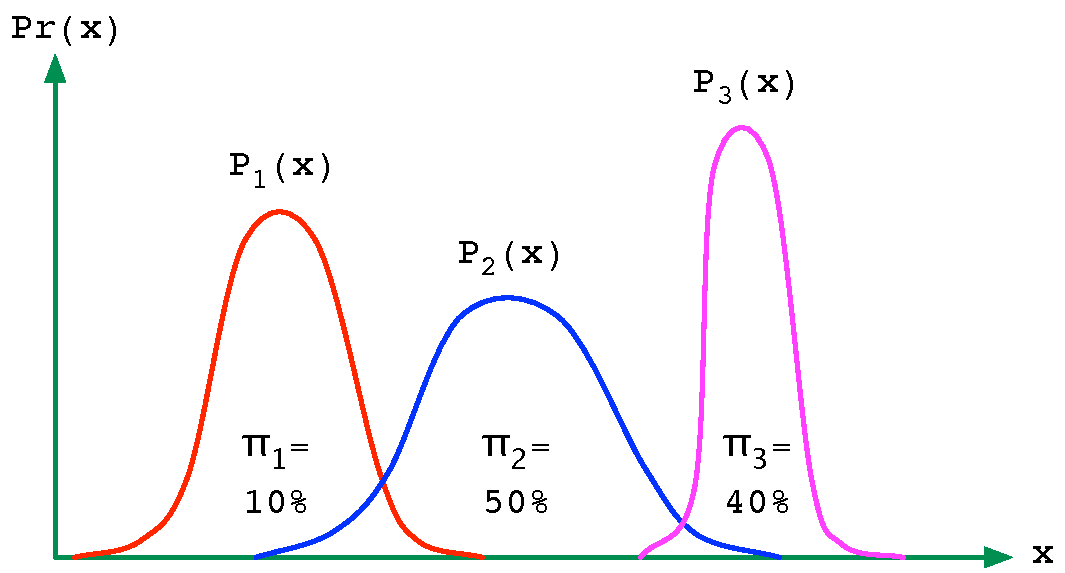
\includegraphics[width=2.75in]{mixture.pdf}
\end{center}

{\darkred Labels $\Y = \{1,2,\ldots,k\}$, density
$\pr(x) = \pi_1 P_1(x) + \cdots + \pi_k P_k(x)$.}

\pause\vone
For any $x \in \X$ and any label $j$,
$$ \pr(y = j | x)
= \frac{\pr(y=j) \pr(x|y=j)}{\pr(x)}
= \frac{\pi_j P_j(x)}{\sum_{i=1}^k \pi_i P_i(x)}
$$
\pause Bayes-optimal prediction:
$h^*(x) = \argmax_j \pi_j P_j(x)$.

\pause\vone
\alert{Estimating the $\pi_j$ is easy. Estimating the $P_j$ is hard.}

\end{frame}

% *** ESTIMATING CLASS-CONDITIONAL DISTRIBUTIONS ***
\begin{frame}
\frametitle{Estimating class-conditional distributions}

{\darkred Estimating an arbitrary distribution in $\R^p$:}
\begin{itemize}
\item {\darkred Can be done, e.g. with kernel density estimation.}
\item {\darkred But number of samples needed is exponential in $p$.}
\end{itemize}

\pause\v2
\alert{Instead: approximate each $P_j$ with a simple, parametric distribution.} 

\pause\v2
Some options:
\begin{itemize}
\item Product distributions.

{\darkgreen Assume coordinates are independent: naive Bayes.}

\item Multivariate Gaussians.

{\darkgreen Linear and quadratic discriminant analysis.}

\item More general graphical models.

\end{itemize}
\end{frame}

% *** THE UNIVARIATE GAUSSIAN ***
\begin{frame}
\frametitle{The univariate Gaussian}

\begin{center}
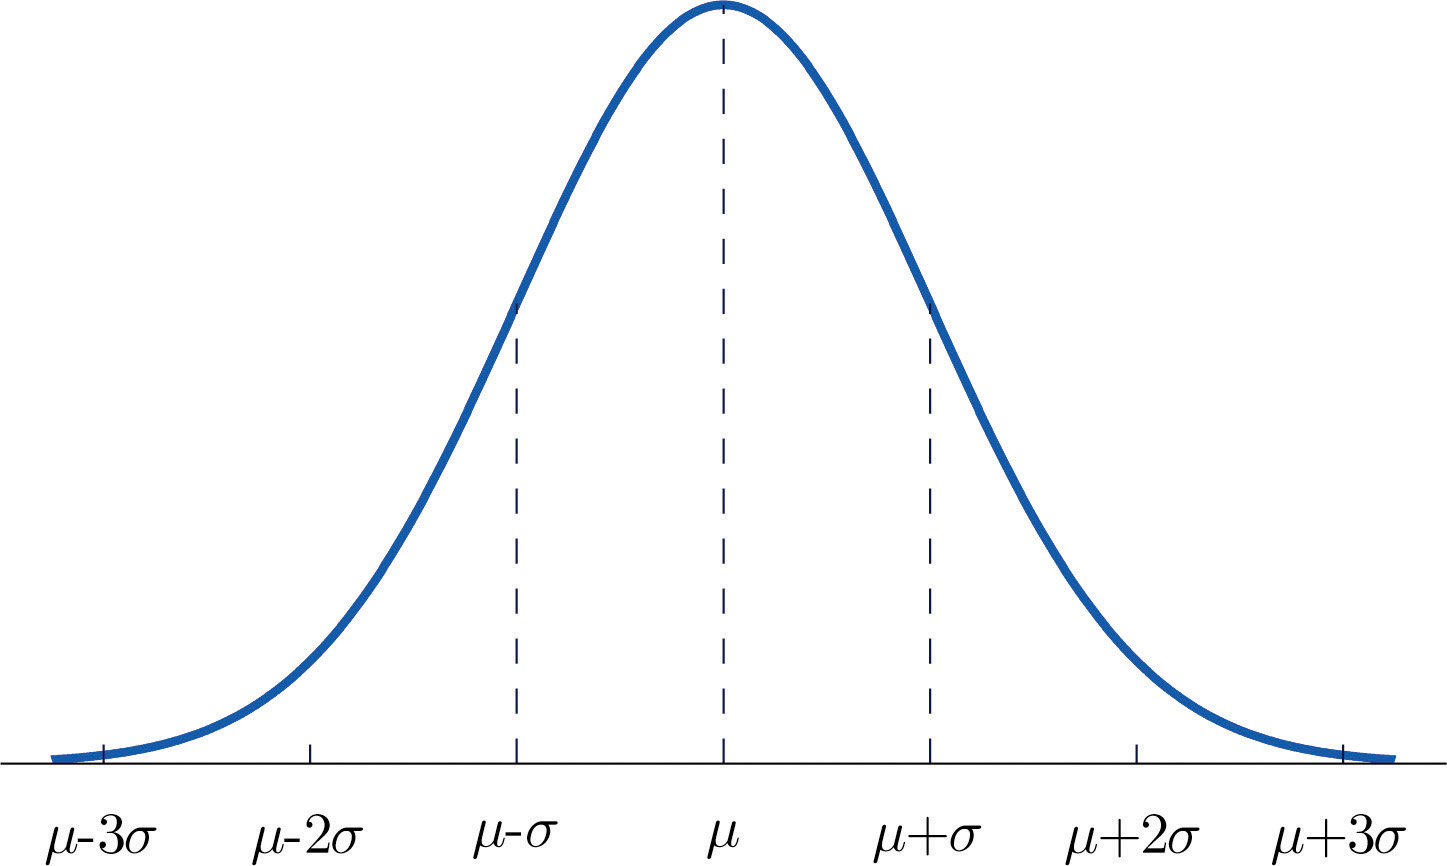
\includegraphics[width=3in]{gaussian1.jpg}
\end{center}

The Gaussian $N(\mu, \sigma^2)$ has mean $\mu$, variance $\sigma^2$, and density function
$$ p(x) = \frac{1}{(2\pi \sigma^2)^{1/2}} \exp \left( - \frac{(x-\mu)^2}{2\sigma^2} \right) .$$

\pause
\alert{But what if we have {\bf two} variables?}

\end{frame}

% *** BIVARIATE DISTRIBUTIONS ***
\begin{frame}
\frametitle{Bivariate distributions}

{\darkred Simplest option: treat each variable as independent.}

\pause\v2
Example: For a large collection of people, measure the two variables
\begin{align*}
H &= \mbox{height} \\
W &= \mbox{weight}
\end{align*}
Independence would mean
$$ \pr(H = h, W = w) \ = \ \pr(H=h) \, \pr(W=w) ,$$
which would also imply $\E(HW) = \E(H) \E(W)$.
 
\pause\v2
\alert{Is this an accurate approximation?}
\pause

\alert{No: we'd expect height and weight to be {\bf positively correlated}.}

\end{frame}

% *** TYPES OF CORRELATION ***
\begin{frame}
\frametitle{Types of correlation}

\hskip.2in
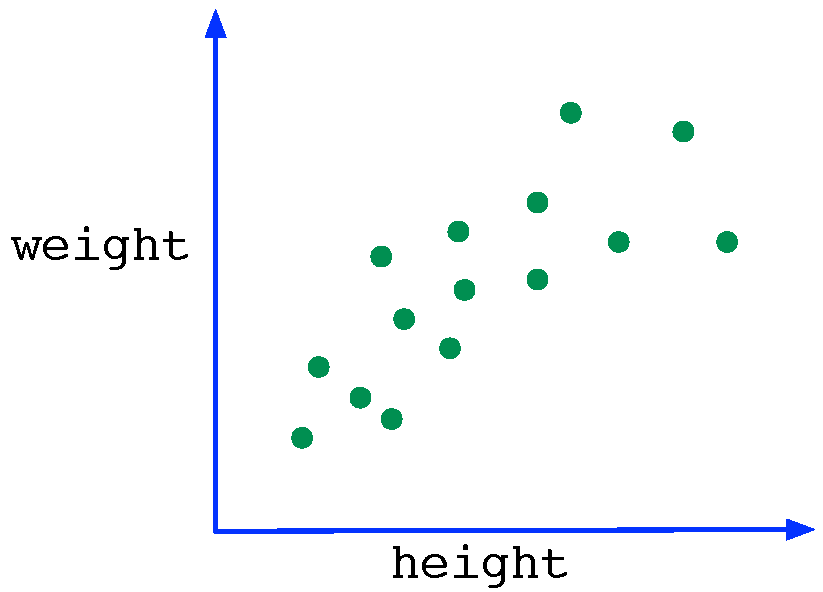
\includegraphics[width=1.75in]{cor1.pdf}
\hskip.25in
\raisebox{.1in}{
\begin{minipage}[b]{1.75in}
{\darkgreen $H,W$ positively correlated.

This also implies 
$$\E(HW) > \E(H) \E(W).$$}
\end{minipage}}

\pause
\begin{columns}
\begin{column}[t]{2in}
\begin{center}
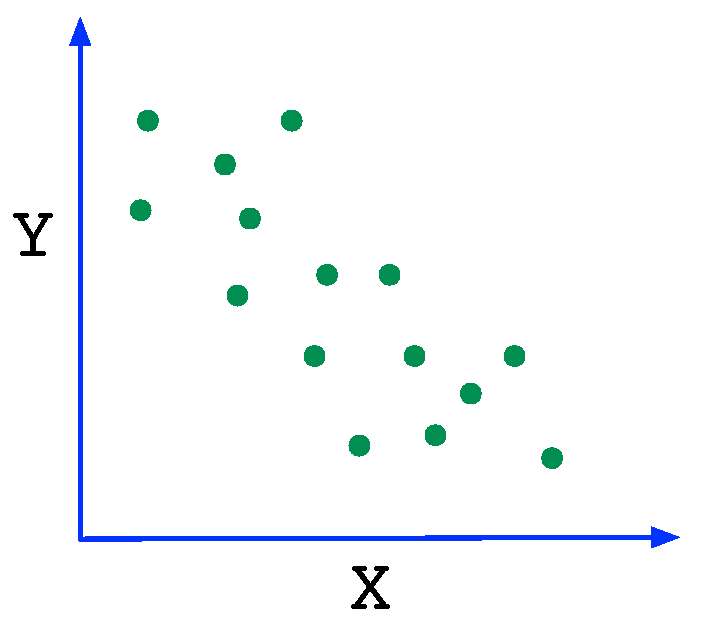
\includegraphics[width=1.5in]{cor2.pdf}

{\darkred \hskip.25in $X,Y$ negatively correlated}
\end{center}
\end{column}
\begin{column}[t]{2in}
\begin{center}
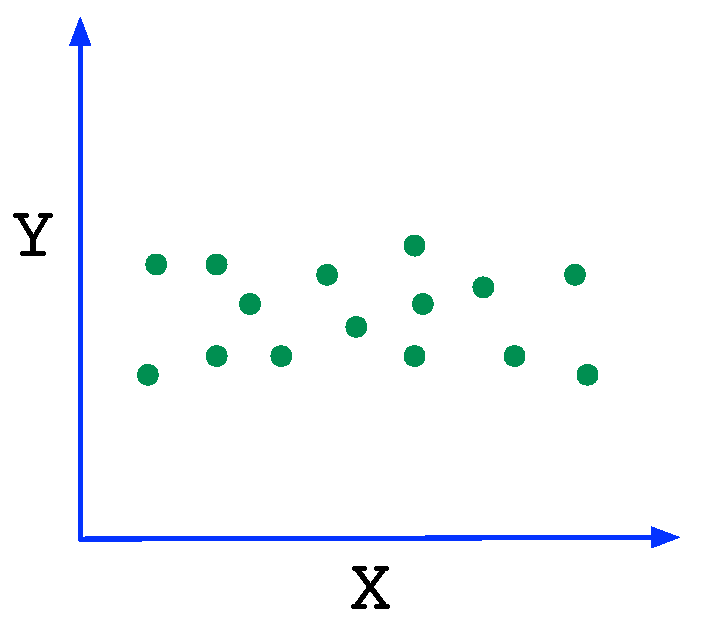
\includegraphics[width=1.5in]{cor3.pdf}

{\darkred \hskip.25in $X,Y$ uncorrelated}
\end{center}
\end{column}
\end{columns}

\end{frame}

% *** PEARSON (1903): FATHERS AND SONS ***
\begin{frame}
\frametitle{Pearson (1903): fathers and sons}

\begin{center}
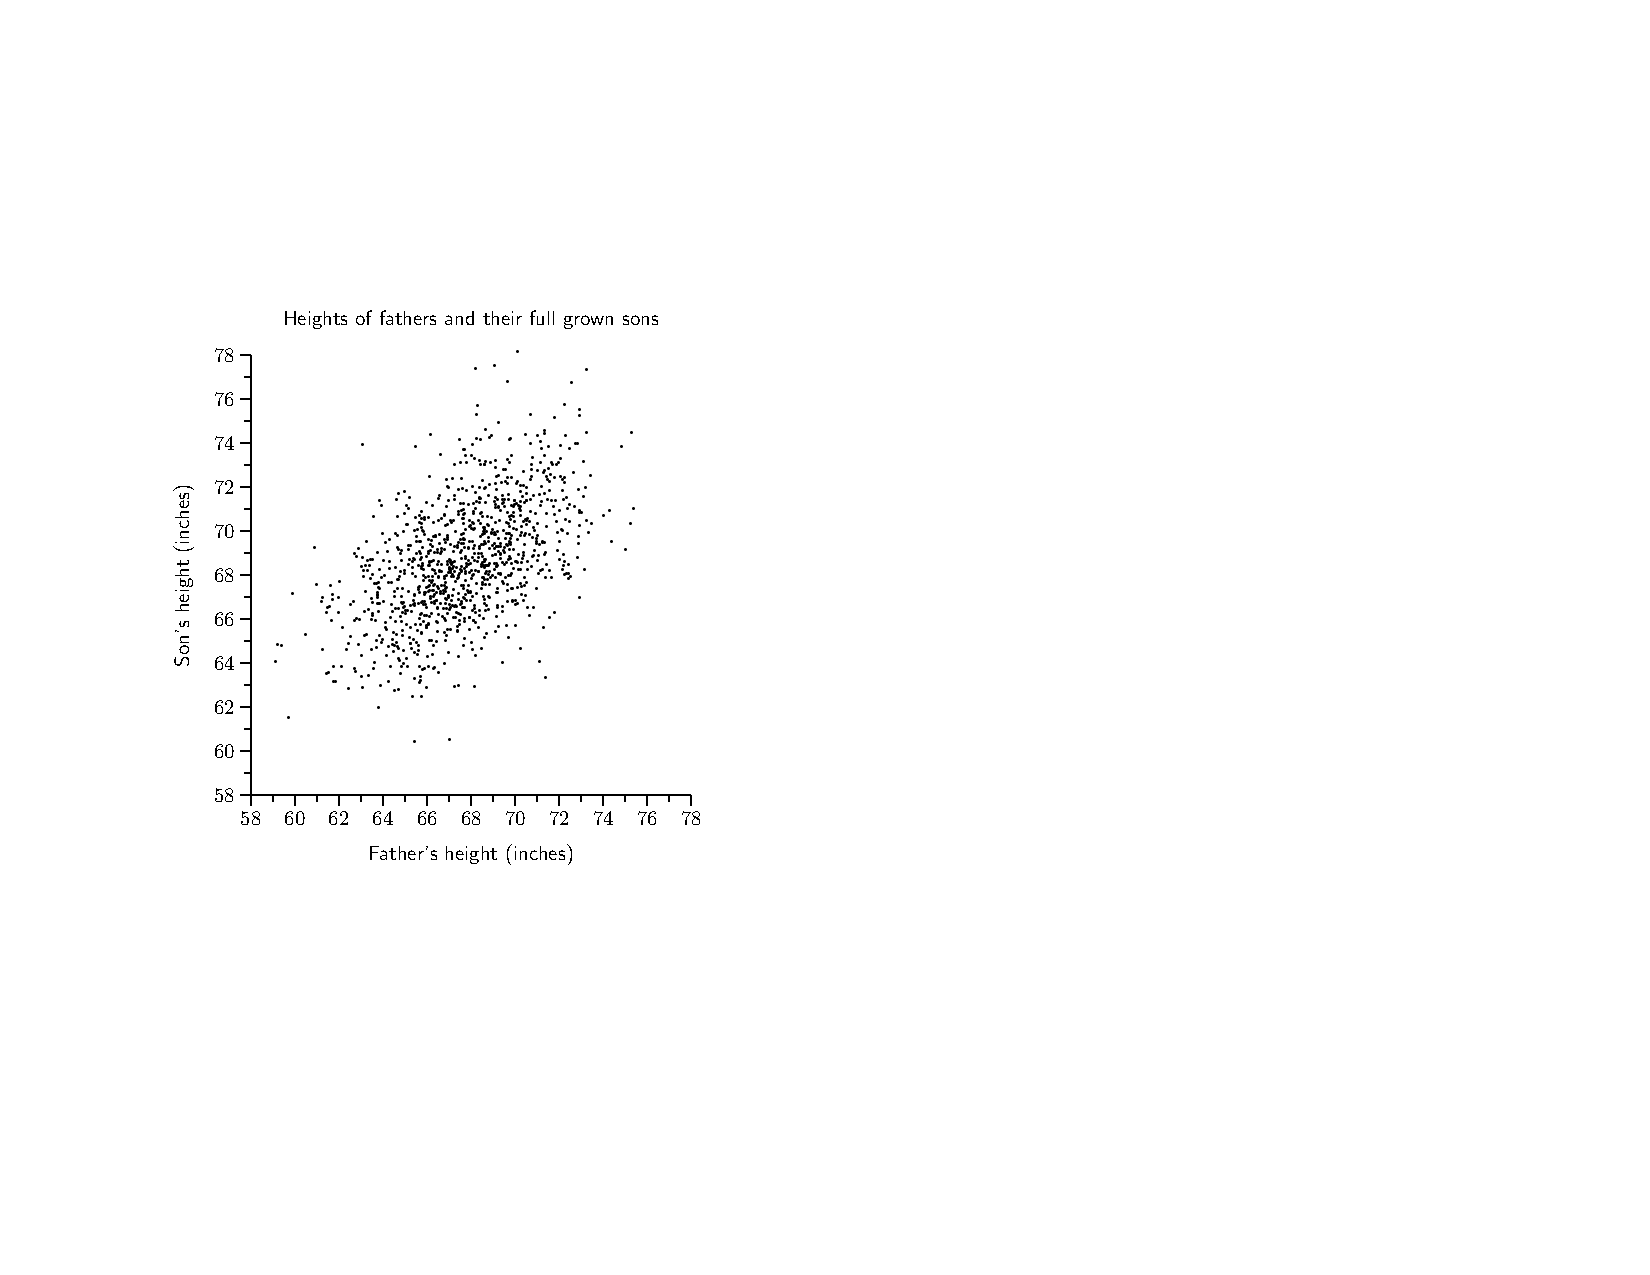
\includegraphics[width=2.75in]{pearson.pdf}
\end{center}

\pause\vskip-.1in
\alert{How to quantify the degree of correlation?}

\end{frame}

% *** CORRELATION PICTURES ***
\begin{frame}
\frametitle{Correlation pictures}

\begin{tabular}{cccc}
\raisebox{.3in}{$r = 0$} & 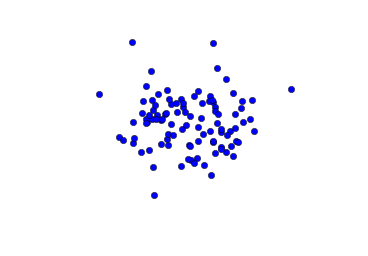
\includegraphics[width=1in]{corr000.png}
&
\raisebox{.3in}{$r = 1$} & 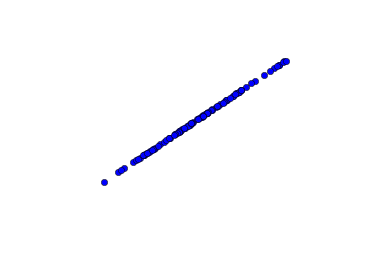
\includegraphics[width=1in]{corr100.png}
\\
\raisebox{.3in}{$r = 0.25$} & 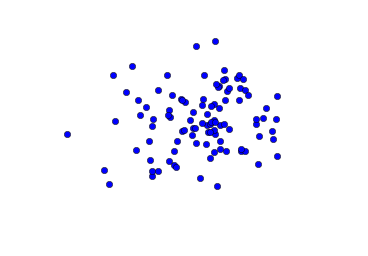
\includegraphics[width=1in]{corr025.png}
&
\raisebox{.3in}{$r = -0.25$} & 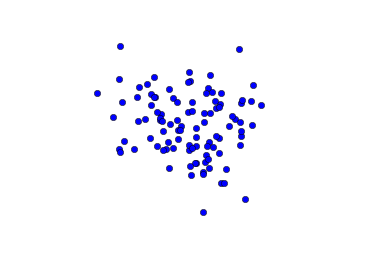
\includegraphics[width=1in]{corr-025.png}
\\
\raisebox{.3in}{$r = 0.5$} & 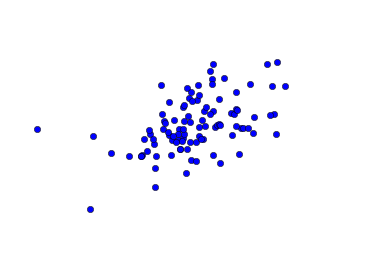
\includegraphics[width=1in]{corr050.png}
&
\raisebox{.3in}{$r = -0.5$} & 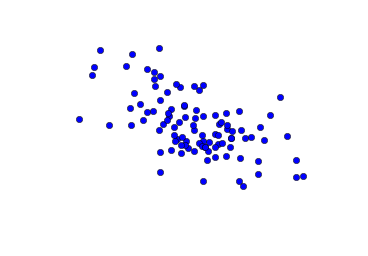
\includegraphics[width=1in]{corr-050.png}
\\
\raisebox{.3in}{$r = 0.75$} & 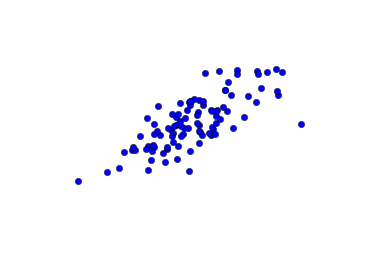
\includegraphics[width=1in]{corr075.png} 
&
\raisebox{.3in}{$r = -0.75$} & 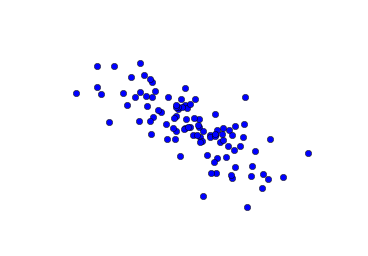
\includegraphics[width=1in]{corr-075.png}
\end{tabular}

\end{frame}

% *** COVARIANCE AND CORRELATION ***
\begin{frame}
\frametitle{Covariance and correlation}

{\darkred Suppose $X$ has mean $\mu_X$ and $Y$ has mean $\mu_Y$.}

\v2
\begin{itemize}
\item \alert{Covariance}
$$ \mbox{cov}(X,Y) = \E [(X-\mu_X)(Y-\mu_Y)] = \E[XY] - \mu_X \mu_Y $$
Maximized when $X=Y$, in which case it is $\mbox{var}(X)$. 

In general, it is at most $\mbox{std}(X) \mbox{std}(Y)$.

\vone
\item<2-> \alert{Correlation}
$$ \mbox{corr}(X,Y) = \frac{\mbox{cov}(X,Y)}{\mbox{std}(X)\mbox{std}(Y)} $$
This is always in the range $[-1,1]$.
\end{itemize}

\end{frame}

% *** COVARIANCE AND CORRELATION: EXAMPLE 1 ***
\begin{frame}
\frametitle{Covariance and correlation: example 1}

\alert{
\begin{align*}
\mbox{cov}(X,Y) 
&= 
\E [(X-\mu_X)(Y-\mu_Y)] \ = \ \E [XY] - \mu_X \mu_Y \\
\mbox{corr}(X,Y) 
&= 
\frac{\mbox{cov}(X,Y)}{\mbox{std}(X)\mbox{std}(Y)}
\end{align*}}


\begin{columns}
\begin{column}[b]{1.5in}
\raisebox{.75in}{
\hskip.5in
\begin{tabular}{ccc}
$x$ & $y$ & $\pr(x,y)$ \\ \hline
$-1$  & $-1$  &  $1/3$ \\ 
$-1$  &  $1$  &  $1/6$ \\
$1$   &  $-1$ &  $1/3$ \\
$1$   &  $1$  &  $1/6$
\end{tabular}}
\end{column}

\begin{column}[b]{3in}
\begin{align*}
\mu_X &= \onslide<2->{0} \\
\mu_Y &= \onslide<2->{-1/3} \\
\mbox{var}(X) &= \onslide<2->{1} \\
\mbox{var}(Y) &= \onslide<2->{8/9} \\
\mbox{cov}(X,Y) &= \onslide<2->{0} \\
\mbox{corr}(X,Y) &= \onslide<2->{0}
\end{align*}
\end{column}
\end{columns}

\v2
\onslide<3->{\darkred
In this case, $X,Y$ are independent. 
Independent variables always have zero
covariance and correlation.}

\end{frame}

% *** COVARIANCE AND CORRELATION: EXAMPLE 2 ***
\begin{frame}
\frametitle{Covariance and correlation: example 2}

\alert{
\begin{align*}
\mbox{cov}(X,Y) 
&= 
\E [(X-\mu_X)(Y-\mu_Y)] \ = \ \E [XY] - \mu_X \mu_Y \\
\mbox{corr}(X,Y) 
&= 
\frac{\mbox{cov}(X,Y)}{\mbox{std}(X)\mbox{std}(Y)}
\end{align*}}


\begin{columns}
\begin{column}[b]{1.5in}
\raisebox{.75in}{
\hskip.5in
\begin{tabular}{ccc}
$x$ & $y$ & $\pr(x,y)$ \\ \hline
$-1$  & $-10$  &  $1/6$ \\ 
$-1$  & $10$   &  $1/3$ \\
$1$   & $-10$  &  $1/3$ \\
$1$   & $10$   &  $1/6$
\end{tabular}}
\end{column}

\begin{column}[b]{3in}
\begin{align*}
\mu_X &= \onslide<2->{0} \\
\mu_Y &= \onslide<2->{0} \\
\mbox{var}(X) &= \onslide<2->{1} \\
\mbox{var}(Y) &= \onslide<2->{100} \\
\mbox{cov}(X,Y) &= \onslide<2->{-10/3} \\
\mbox{corr}(X,Y) &= \onslide<2->{-1/3}
\end{align*}
\end{column}
\end{columns}

\v2
\onslide<3->{\darkred
In this case, $X$ and $Y$ are negatively correlated.
\\
}
\end{frame}

% *** THE BIVARIATE (2-D) GAUSSIAN ***
\begin{frame}
\frametitle{The bivariate (2-d) Gaussian}

{\darkred A distribution over $(x,y) \in \R^2$, parametrized by:}
\begin{itemize}
\item {\darkred {\bf Mean} $(\mu_x, \mu_y) \in \R^2$}
\item {\darkred {\bf Covariance matrix}
$$ \Sigma = 
\left[ 
\begin{array}{cc}
\Sigma_{xx} & \Sigma_{xy} \\
\Sigma_{yx} & \Sigma_{yy}
\end{array}
\right]
$$
where
$\Sigma_{xx} = \mbox{var}(X), 
\ \Sigma_{yy} = \mbox{var}(Y), 
\ \Sigma_{xy} = \Sigma_{yx} = \mbox{cov}(X,Y)$}
\end{itemize}

\pause
$$ \mbox{Density\ \ }p(x,y) = \frac{1}{2\pi |\Sigma|^{1/2}} 
\exp\left(- \frac{1}{2} 
\left[
\begin{array}{c}
x-\mu_x \\ 
y-\mu_y
\end{array}
\right]^T
\Sigma^{-1}
\left[
\begin{array}{c}
x-\mu_x \\ 
y-\mu_y
\end{array}
\right]
 \right) $$

\pause
\vskip-.2in
\raisebox{.7in}{
\begin{minipage}[b]{2in}
\alert{The density is highest at the mean, and falls off in ellipsoidal contours.}
\end{minipage}}
\hskip.2in
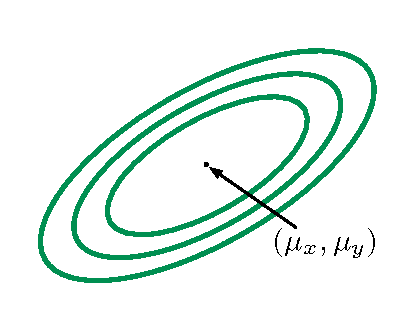
\includegraphics[width=1.7in]{gauss2d.pdf}

\end{frame}

% *** BIVARIATE GAUSSIAN: EXAMPLES ***
\begin{frame}
\frametitle{Bivariate Gaussian: examples}

{\darkred In either case, the mean is $(1,1)$.}

\v2
\begin{columns}
\begin{column}[t]{2in}

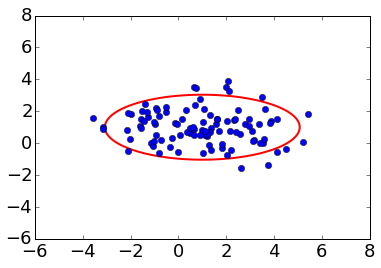
\includegraphics[width=2in]{gaussian2d-1.png}

$$\Sigma = 
\left[
\begin{array}{cc}
4 & 0 \\
0 & 1
\end{array}
\right]
$$

\end{column}
\begin{column}[t]{2in}

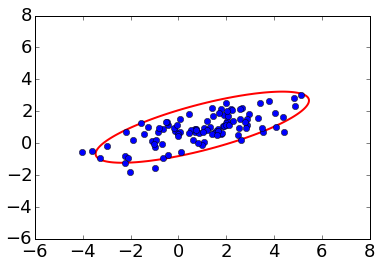
\includegraphics[width=2in]{gaussian2d-2.png}

$$\Sigma = 
\left[
\begin{array}{cc}
4 & 1.5 \\
1.5 & 1
\end{array}
\right]
$$

\end{column}
\end{columns}

\end{frame}

% *** THE MULTIVARIATE GAUSSIAN ***
\begin{frame}
\frametitle{The multivariate Gaussian}

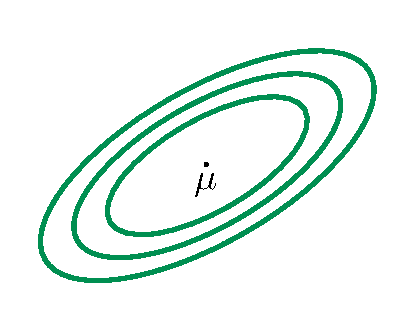
\includegraphics[width=1.75in]{gaussian2.pdf}
\hskip.1in
\raisebox{.5in}{
\begin{minipage}[b]{2in}
{\darkred $N(\mu,\Sigma)$: Gaussian in $\R^p$}
\begin{itemize}
\item {\darkred mean:  $\mu \in \R^p$}
\item {\darkred covariance: $p \times p$ matrix $\Sigma$}
\end{itemize}
\end{minipage}}

\vskip-.25in
{\darkred $$ \mbox{Density\ \ \ } p(x) = \frac{1}{(2\pi)^{p/2} |\Sigma|^{1/2}} \exp\left(- \frac{1}{2} (x-\mu)^T \Sigma^{-1} (x-\mu) \right) $$}

\vone
\alert{Let $X = (X_1, X_2, \ldots, X_p)$ be a random draw from $N(\mu,\Sigma)$.}
\begin{itemize}
\item $\mu$ is the vector of coordinate-wise means:
$$ \mu_1 = \E X_1, \ \mu_2 = \E X_2, \ldots,\ \mu_p = \E X_p .$$
\item $\Sigma$ is a matrix containing all pairwise covariances:
\begin{align*}
\Sigma_{ij} = \Sigma_{ji} &= \mbox{cov}(X_i, X_j) \mbox{\ \ \ \ if $i \neq j$} \\
\Sigma_{ii} &= \mbox{var}(X_i) 
\end{align*}
\item In matrix/vector form: $\mu = \E X$ and $\Sigma = \E (X-\mu)(X-\mu)^T$.
\end{itemize}
\end{frame}

% *** SPECIAL CASE: SPHERICAL GAUSSIAN ***
\begin{frame}
\frametitle{Special case: spherical Gaussian}

{\darkred The $X_i$ are independent and all have the same variance $\sigma^2$. Thus
$$ \Sigma = \sigma^2 I_p = \mbox{diag}(\sigma^2, \sigma^2, \ldots, \sigma^2)$$
(off-diagonal elements zero, diagonal elements $\sigma^2$).}

\pause\v2
Each $X_i$ is an independent univariate Gaussian $N(\mu_i,\sigma^2)$:
$$ 
\pr(x) 
\ = \ 
\prod_{i=1}^p \left(\frac{1}{\sigma \sqrt{2\pi}} e^{-(x_i-\mu_i)^2/2\sigma^2} \right)
= 
\frac{1}{(2\pi)^{p/2} \sigma^p} \exp\left( - \frac{\|x-\mu\|^2}{2\sigma^2} \right) $$

\pause\vone

\raisebox{.7in}{
\begin{minipage}[t]{2in}
\alert{Density at a point depends only on its distance from $\mu$:}
\end{minipage}}
\hskip.4in

\includegraphics[width=1.1in]{gaussian3.pdf}

\end{frame}

% *** SPECIAL CASE: DIAGONAL GAUSSIAN ***
\begin{frame}
\frametitle{Special case: diagonal Gaussian}

{\darkred The $X_i$ are independent, with variances $\sigma_i^2$. Thus
$$ \Sigma = \mbox{diag}(\sigma_1^2, \ldots, \sigma_p^2) $$
(all off-diagonal elements zero).}

\pause\v2
Each $X_i$ is an independent univariate Gaussian $N(\mu_i, \sigma_i^2)$:
$$ p(x) = \frac{1}{(2\pi)^{p/2} \sigma_1 \cdots \sigma_p} 
\exp\left( - \sum_{i=1}^p \frac{(x_i - \mu_i)^2}{2 \sigma_i^2} \right) $$

\pause\vone
\raisebox{.6in}{
\begin{minipage}[t]{2in}
\alert{Contours of equal density are axis-aligned ellipsoids centered at $\mu$:}
\end{minipage}}
\hskip.2in
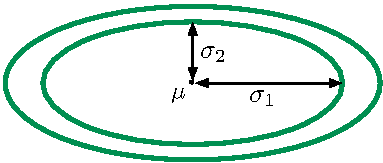
\includegraphics[width=1.75in]{gaussian5.pdf}

\end{frame}

% *** THE GENERAL GAUSSIAN ***
\begin{frame}
\frametitle{The general Gaussian $N(\mu,\Sigma)$ in $\R^p$}

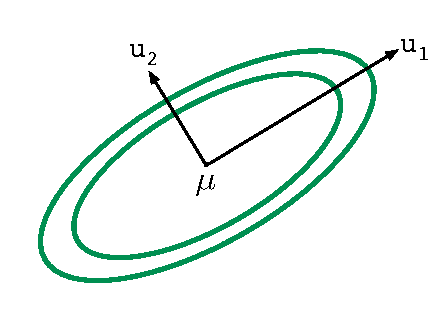
\includegraphics[width=1.75in]{gaussian6.pdf}
\hskip.25in\pause
\raisebox{1.2in}{\begin{minipage}[t]{2in}
{\darkred Eigendecomposition of $\Sigma$ yields:}
\begin{itemize}
\item {\darkred {\bf Eigenvalues} $\lambda_1 \geq \lambda_2 \geq \cdots \geq \lambda_p$}
\item {\darkred Corresponding {\bf eigenvectors} $u_1, \ldots, u_p$}
\end{itemize}
\end{minipage}}

\vskip-.2in\pause
$$ \mbox{Recall density:\ \ \ \ \ } p(x) = \frac{1}{(2\pi)^{p/2} |\Sigma|^{1/2}} \exp\left(- \frac{1}{2}
  \underbrace{(x-\mu)^T \Sigma^{-1} (x-\mu)}_\text{What is this?}
\right) $$
\pause
If we write $S = \Sigma^{-1}$ then $S$ is a $p \times p$ matrix and
$$ (x-\mu)^T \Sigma^{-1} (x-\mu) \ = \ \sum_{i,j} S_{ij} (x_i - \mu_i)(x_j - \mu_j),$$
a {\bf quadratic function} of $x$.
\end{frame}

% *** BINARY CLASSIFICATION WITH GAUSSIAN GENERATIVE MODEL ***
\begin{frame}
\frametitle{Binary classification with Gaussian generative model}

Estimate class probabilities $\pi_1, \pi_2$ and fit a Gaussian to each class: 
$$P_1 = N(\mu_1, \Sigma_1), \ \ P_2 = N(\mu_2, \Sigma_2)$$
{\darkgreen E.g. If data points $x^{(1)}, \ldots, x^{(m)} \in \R^p$ are class 1:
$$
\mu_1 
\ = \  
\frac{1}{m} \left( x^{(1)} + \cdots + x^{(m)} \right)
\mbox{\ \ and\ \ }
\Sigma_1
\ =\ 
\frac{1}{m} \sum_{i=1}^m (x^{(i)} - \mu_1)(x^{(i)}-\mu_1)^T 
$$}

\pause
{\darkred Given a new point $x$, predict class 1 iff:
$$ 
\pi_1 P_1(x) > \pi_2 P_2(x) 
\onslide<3->{\ \ \Leftrightarrow \ \ x^T M x + 2 w^T x \geq \theta,}$$
\onslide<3->{where:
\begin{align*}
M &= \frac{1}{2}(\Sigma_2^{-1} - \Sigma_1^{-1}) \\
w &= \Sigma_1^{-1} \mu_1 - \Sigma_2^{-1} \mu_2 
\end{align*}
and $\theta$ is a constant depending on the various parameters.}}

\vone
\onslide<4->{\alert{$\Sigma_1 = \Sigma_2$: {\bf linear} decision boundary. 
Otherwise, {\bf quadratic} boundary.}}
\end{frame}

% *** LINEAR DECISION BOUNDARY ***
\begin{frame}
\frametitle{Linear decision boundary}

When $\Sigma_1 = \Sigma_2 = \Sigma$: choose class 1 iff 
$$ x \ \cdot \ \underbrace{\Sigma^{-1}(\mu_1 - \mu_2)}_{w} \ \geq \ \theta .$$

\pause
{\darkgreen What does $x \cdot w$ (or equivalently $x^T w$, or $w^T x$) mean?}

\pause
\begin{flalign*}& \mbox{\darkred Algebraically:\ \ } x \cdot w = w \cdot x = x^T w = w^T x = \sum_{i=1}^p x_i w_i &\end{flalign*}

\pause
    {\darkred Geometrically:}
    \alert{Suppose $w$ is a unit vector (that is, $\|w\| = 1$). Then
$x \cdot w$ is the projection of vector $x$ onto direction $w$.}

\begin{center}
  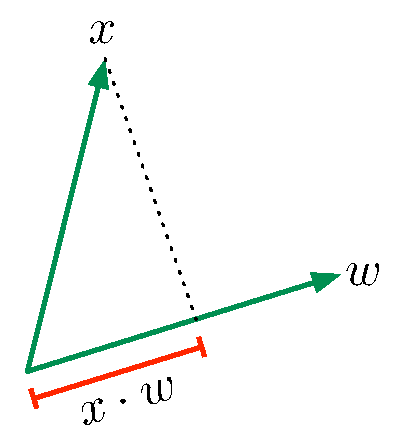
\includegraphics[width=1.25in]{projection.pdf}
\end{center}

\end{frame}

% *** LINEAR DECISION BOUNDARY ***
\begin{frame}
\frametitle{Linear decision boundary}

Let $w$ be any vector in $\R^p$. What is meant by decision rule
$w \cdot x \geq \theta$ ?


\begin{center}
  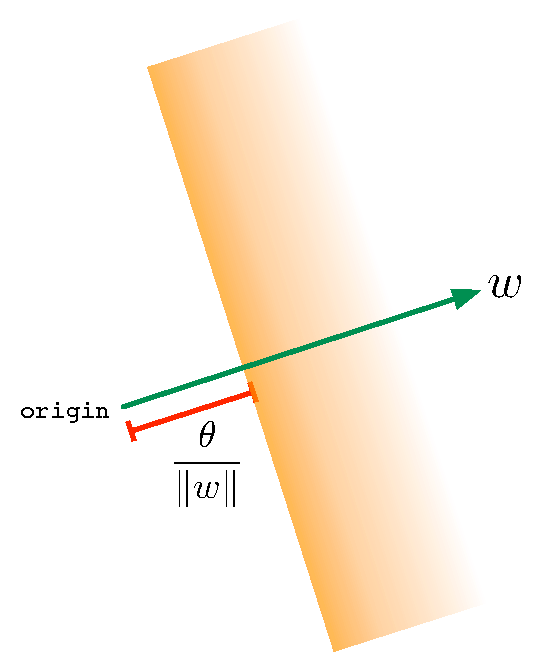
\includegraphics[width=2in]{projection2.pdf}
\end{center}

\end{frame}

% *** COMMON COVARIANCE: $\Sigma_1 = \Sigma_2$ ***
\begin{frame}
\frametitle{Common covariance: $\Sigma_1 = \Sigma_2 = \Sigma$}
  
\alert{Linear decision boundary: choose class 1 iff 
$$ x \ \cdot \ \underbrace{\Sigma^{-1}(\mu_1 - \mu_2)}_{w} \ \geq \ \theta .$$}

\pause
{\darkred Example 1: Spherical Gaussians with $\Sigma = I_p$ and $\pi_1 = \pi_2$.}

\vone
\begin{center}
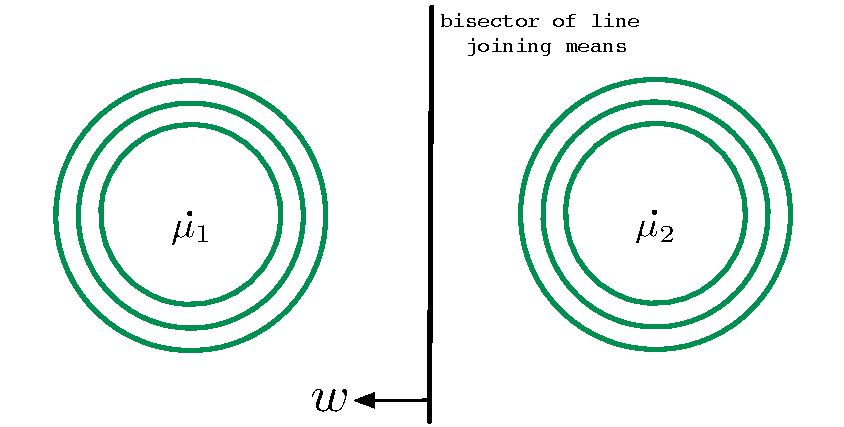
\includegraphics[width=3in]{discriminant1.pdf}
\end{center}

\end{frame}

%

\begin{frame}

{\darkred Example 2: Again spherical, but now $\pi_1 > \pi_2$.}

\pause\vone
\begin{center}
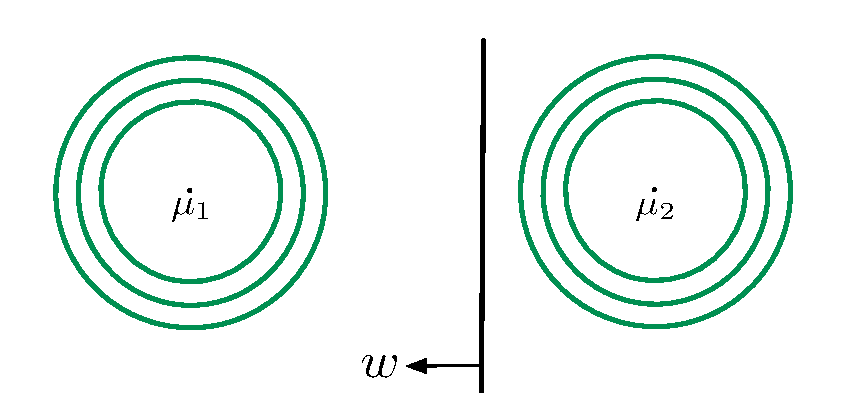
\includegraphics[width=3in]{discriminant2.pdf}
\end{center}

\pause\vone
\alert{One-d projection onto $w$:}

\vone
\begin{center}
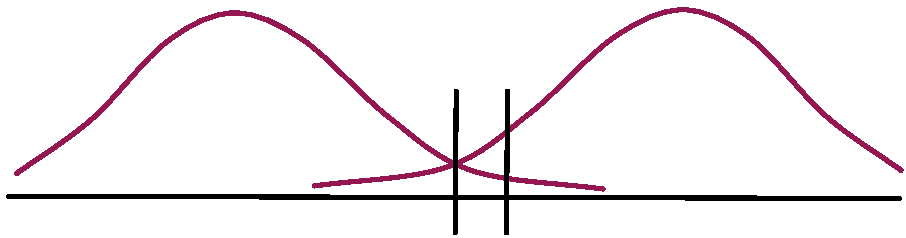
\includegraphics[width=3in]{discriminant3.pdf}
\end{center}

\end{frame}

%

\begin{frame}

{\darkred Example 3: Non-spherical.}

\begin{center}
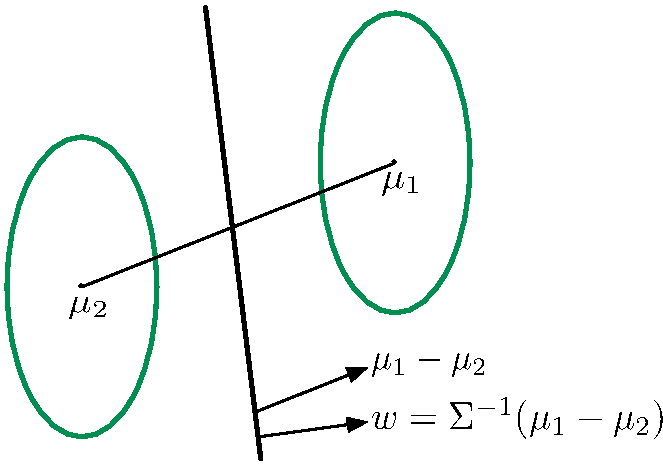
\includegraphics[width=3in]{discriminant4.pdf}
\end{center}

\pause\vone
\alert{Rule: $w \cdot x \geq \theta$}
\begin{itemize}
\item $w,\theta$ dictated by probability model, assuming it is a perfect fit
\item Common practice: choose $w$ as above, but fit $\theta$ to minimize training/validation error
\end{itemize}

\end{frame}

% *** DIFFERENT COVARIANCES ***
\begin{frame}
\frametitle{Different covariances: $\Sigma_1 \neq \Sigma_2$}

\alert{Quadratic boundary: choose class 1 iff 
$x^T M x + 2 w^T x \geq \theta$, where:
\begin{align*}
M &= \frac{1}{2}(\Sigma_2^{-1} - \Sigma_1^{-1}) \\
w &= \Sigma_1^{-1} \mu_1 - \Sigma_2^{-1} \mu_2 
\end{align*}}

{\darkred Example 1: $\Sigma_1 = \sigma_1^2 I_p$ and $\Sigma_2 = \sigma_2^2 I_p$ with $\sigma_1 > \sigma_2$}

\begin{center}
\includegraphics<1>[width=3.5in]{discriminant6.pdf}
\includegraphics<2->[width=3.5in]{discriminant5.pdf}
\end{center}

\end{frame}
%

\begin{frame}

{\darkred Example 2: Same thing in 1-d. $\X = \R$.}

\begin{center}
\includegraphics<1>[width=3.5in]{discriminant8.pdf}
\includegraphics<2->[width=3.5in]{discriminant7.pdf}
\end{center}

\end{frame}

%

\begin{frame}

{\darkred Example 3: A parabolic boundary.}

\begin{center}
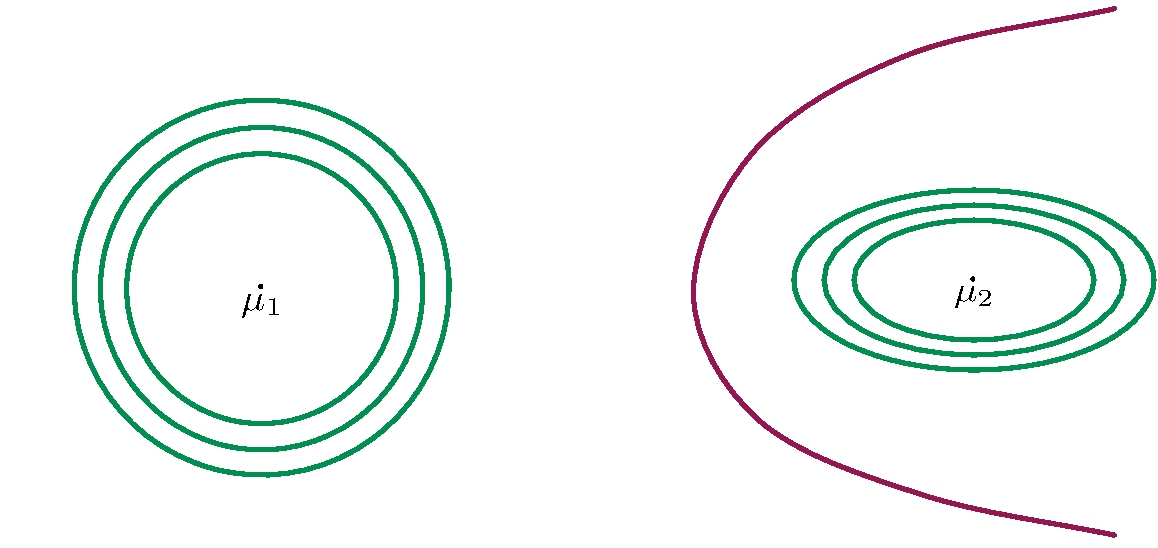
\includegraphics[width=4in]{discriminant9.pdf}
\end{center}

\pause\alert{Many other possibilities!}

\end{frame}

% *** MULTICLASS DISCRIMINANT ANALYSIS ***
\begin{frame}
\frametitle{Multiclass discriminant analysis}

{\darkred $k$ classes: weights $\pi_j$, class-conditional distributions $P_j = N(\mu_j, \Sigma_j)$.}

\pause\v2
Each class has an associated {\bf quadratic} function
$$ f_j(x) = \log \left( \pi_j \, P_j(x) \right) $$ 
To class a point $x$, pick $\argmax_j f_j(x)$.

\pause\v2
\alert{If $\Sigma_1 = \cdots = \Sigma_k$, the boundaries are {\bf linear}.}

\begin{center}
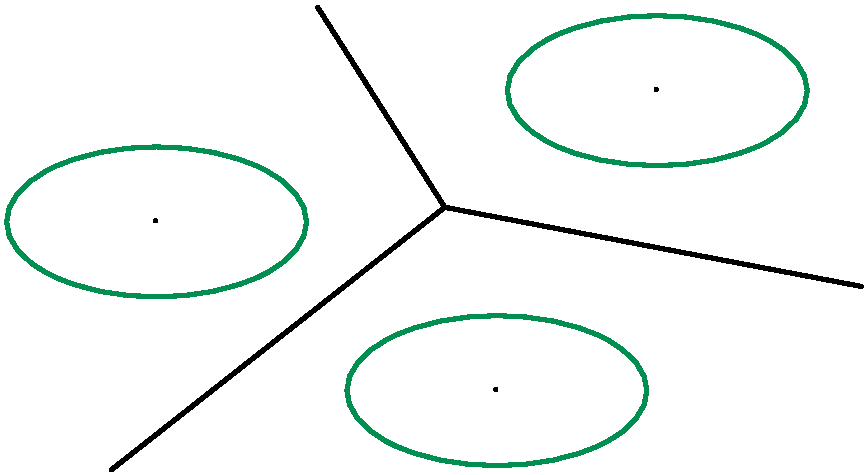
\includegraphics[width=2.5in]{discriminant10.pdf}
\end{center}

\end{frame}

% *** EXAMPLE: WINE DATA SET ***
\begin{frame}
\frametitle{Example: ``wine'' data set}

{\darkred Data from three wineries from the same region of Italy}
\begin{itemize}
\item 13 attributes: hue, color intensity, flavanoids, ash content, ...
\item 178 instances in all: split into 118 train, 60 test
\end{itemize}

\begin{center}
\includegraphics<1>[width=3in]{wine.png}
\includegraphics<2->[width=3in]{wine2.png}
\end{center}

\onslide<3->{\darkgreen Test error using multiclass discriminant analysis: 1/60}

\end{frame}

% *** EXAMPLE: MNIST ***
\begin{frame}
\frametitle{Example: MNIST}

\hskip.1in
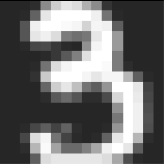
\includegraphics[width=1in]{mnist1.jpg}
\hskip.1in
\raisebox{.2in}{
\begin{minipage}[b]{2.8in}
{\darkgreen To each digit, fit:}
\begin{itemize}
\item {\darkgreen class probability $\pi_j$}
\item {\darkgreen mean $\mu_j \in \R^{784}$}
\item {\darkgreen covariance matrix $\Sigma_j \in \R^{784\times784}$}
\end{itemize}
\end{minipage}
}

\pause\v2
\alert{Problem: formula for normal density uses $\Sigma_j^{-1}$, which is singular.}
\begin{itemize}
\item<3-> Need to {\bf regularize/smooth}: $\Sigma_j \rightarrow \Sigma_j + \sigma^2 I$
\item<4-> This is a good idea even without the singularity issue
\end{itemize}

\v2
\onslide<5->{\darkred How to choose $c$? With a {\bf validation set}.
\begin{itemize}
\item Divide original training set into a training set and a validation set.
\item Fit parameters $\pi_j, \mu_j, \Sigma_j$ to training set
\item Choose the constant $c$ that yields lowest error rate on validation set
\end{itemize}}

\end{frame}

% *** FISHER'S LINEAR DISCRIMINANT ***
\begin{frame}
\frametitle{Fisher's linear discriminant}

{\darkred A framework for linear classification without Gaussian assumptions.}

\pause\v2
{\darkgreen Use only first- and second-order statistics of the classes.

\begin{center}
\begin{tabular}{c|c}
Class 1 & Class 2 \\ \hline
mean $\mu_1$ & mean $\mu_2$ \\
cov $\Sigma_1$ & cov $\Sigma_2$ \\
\# pts $n_1$ & \# pts $n_2$
\end{tabular}
\end{center}}

\pause\v2
A linear classifier projects all data onto a direction $w$. Choose $w$
so that:
\begin{itemize}
\item<4-> Projected means are well-separated, i.e. $(w \cdot \mu_1 - w \cdot \mu_2)^2$ is large.
\item<5-> Projected within-class variance is small.
\end{itemize}

\onslide<5->{
\begin{center}
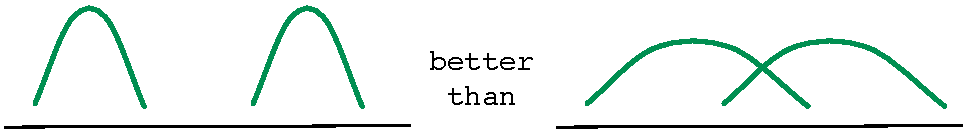
\includegraphics[width=4in]{fisher1.pdf}
\end{center}}

\end{frame}

% *** FISHER LDA ***
\begin{frame}
\frametitle{Fisher LDA (linear discriminant analysis)}

{\darkgreen Two classes: means $\mu_1, \mu_2$; covariances $\Sigma_1, \Sigma_2$; sample sizes $n_1, n_2$.}

\pause\vone
{\darkred Project data onto direction (unit vector) $w$.}
\begin{itemize}
\item Projected means: $w \cdot \mu_1$ and $w \cdot \mu_2$
\item Projected variances: $w^T \Sigma_1 w$ and $w^T \Sigma_2 w$
\item Average projected variance:
$$ \frac{n_1 (w^T \Sigma_1 w) + n_2 (w^T \Sigma_2 w)}{n_1+n_2} = w^T \Sigma w,$$
where $\Sigma = (n_1 \Sigma_1 + n_2 \Sigma_2)/(n_1 + n_2)$.
\end{itemize}
\alert{
\begin{flalign*} 
\onslide<3->{&\mbox{Find $w$ to maximize\ \ } J(w) = \frac{(w \cdot \mu_1 - w \cdot \mu_2)^2}{w^T \Sigma w}& \\}
\onslide<4->{\\&\mbox{Solution:\ \ } w \propto \Sigma^{-1}(\mu_1 - \mu_2). \mbox{\ \ Look familiar?}&}
\end{flalign*}
}
\end{frame}


\end{document}
